%=============================================================================
\section{Experimental Results}\label{sec:resultModel}

We used $T_k$ values computed as described in Section~\ref{sec:proposeModel}. We have performed experiments to evaluate the predictions of our model, by comparing these predictions with measurements of executions of the applications over different GPUs showed in Table~\ref{tab:GPUs}. For all simulations, we considered $5$ cycles for latency in the communication in shared memory and $500$ cycles are considered for latency communication in global memory \citep{CUDA:Best}. Finally, for the parameter $\lambda$, which captures the effects of thread divergence, global memory access optimizations, and shared memory bank conflicts, we used the values described in the previous section. We compared the measured times ($T_m$) with the times predicted by the proposed model ($T_k$), and used the ratio $T_k/T_m$ to define the precision of the prediction. 

Figure~\ref{fig:resultsVMApp} and \ref{fig:ResultsRodinia} show the obtained results for the vector/matrix applications and some Rodinia Kernels. These figures show the box plots of the accuracy of the BSP-based analytical model over the different selected CUDA kernels. The box plots show the median for each GPU and the upper and lower first quartiles, with whiskers representing the 95\% confidence interval. Outliers are marked as individual points. For vector/matrix applications in the \ref{fig:resultsVMApp}, the predicted execution time was within 10\% of the measured time ($T_k/T_m$ between 0.9 and 1.1). We consider this an excellent result, considering that all the complexity in the memory and thread hierarchy was adjusted using a single parameter $\lambda$. Moreover, this ratio remained nearly constant for all input sizes, which shows that the prediction accuracy is dependent of the problem size.

\begin{figure}[htpb]
\centering
 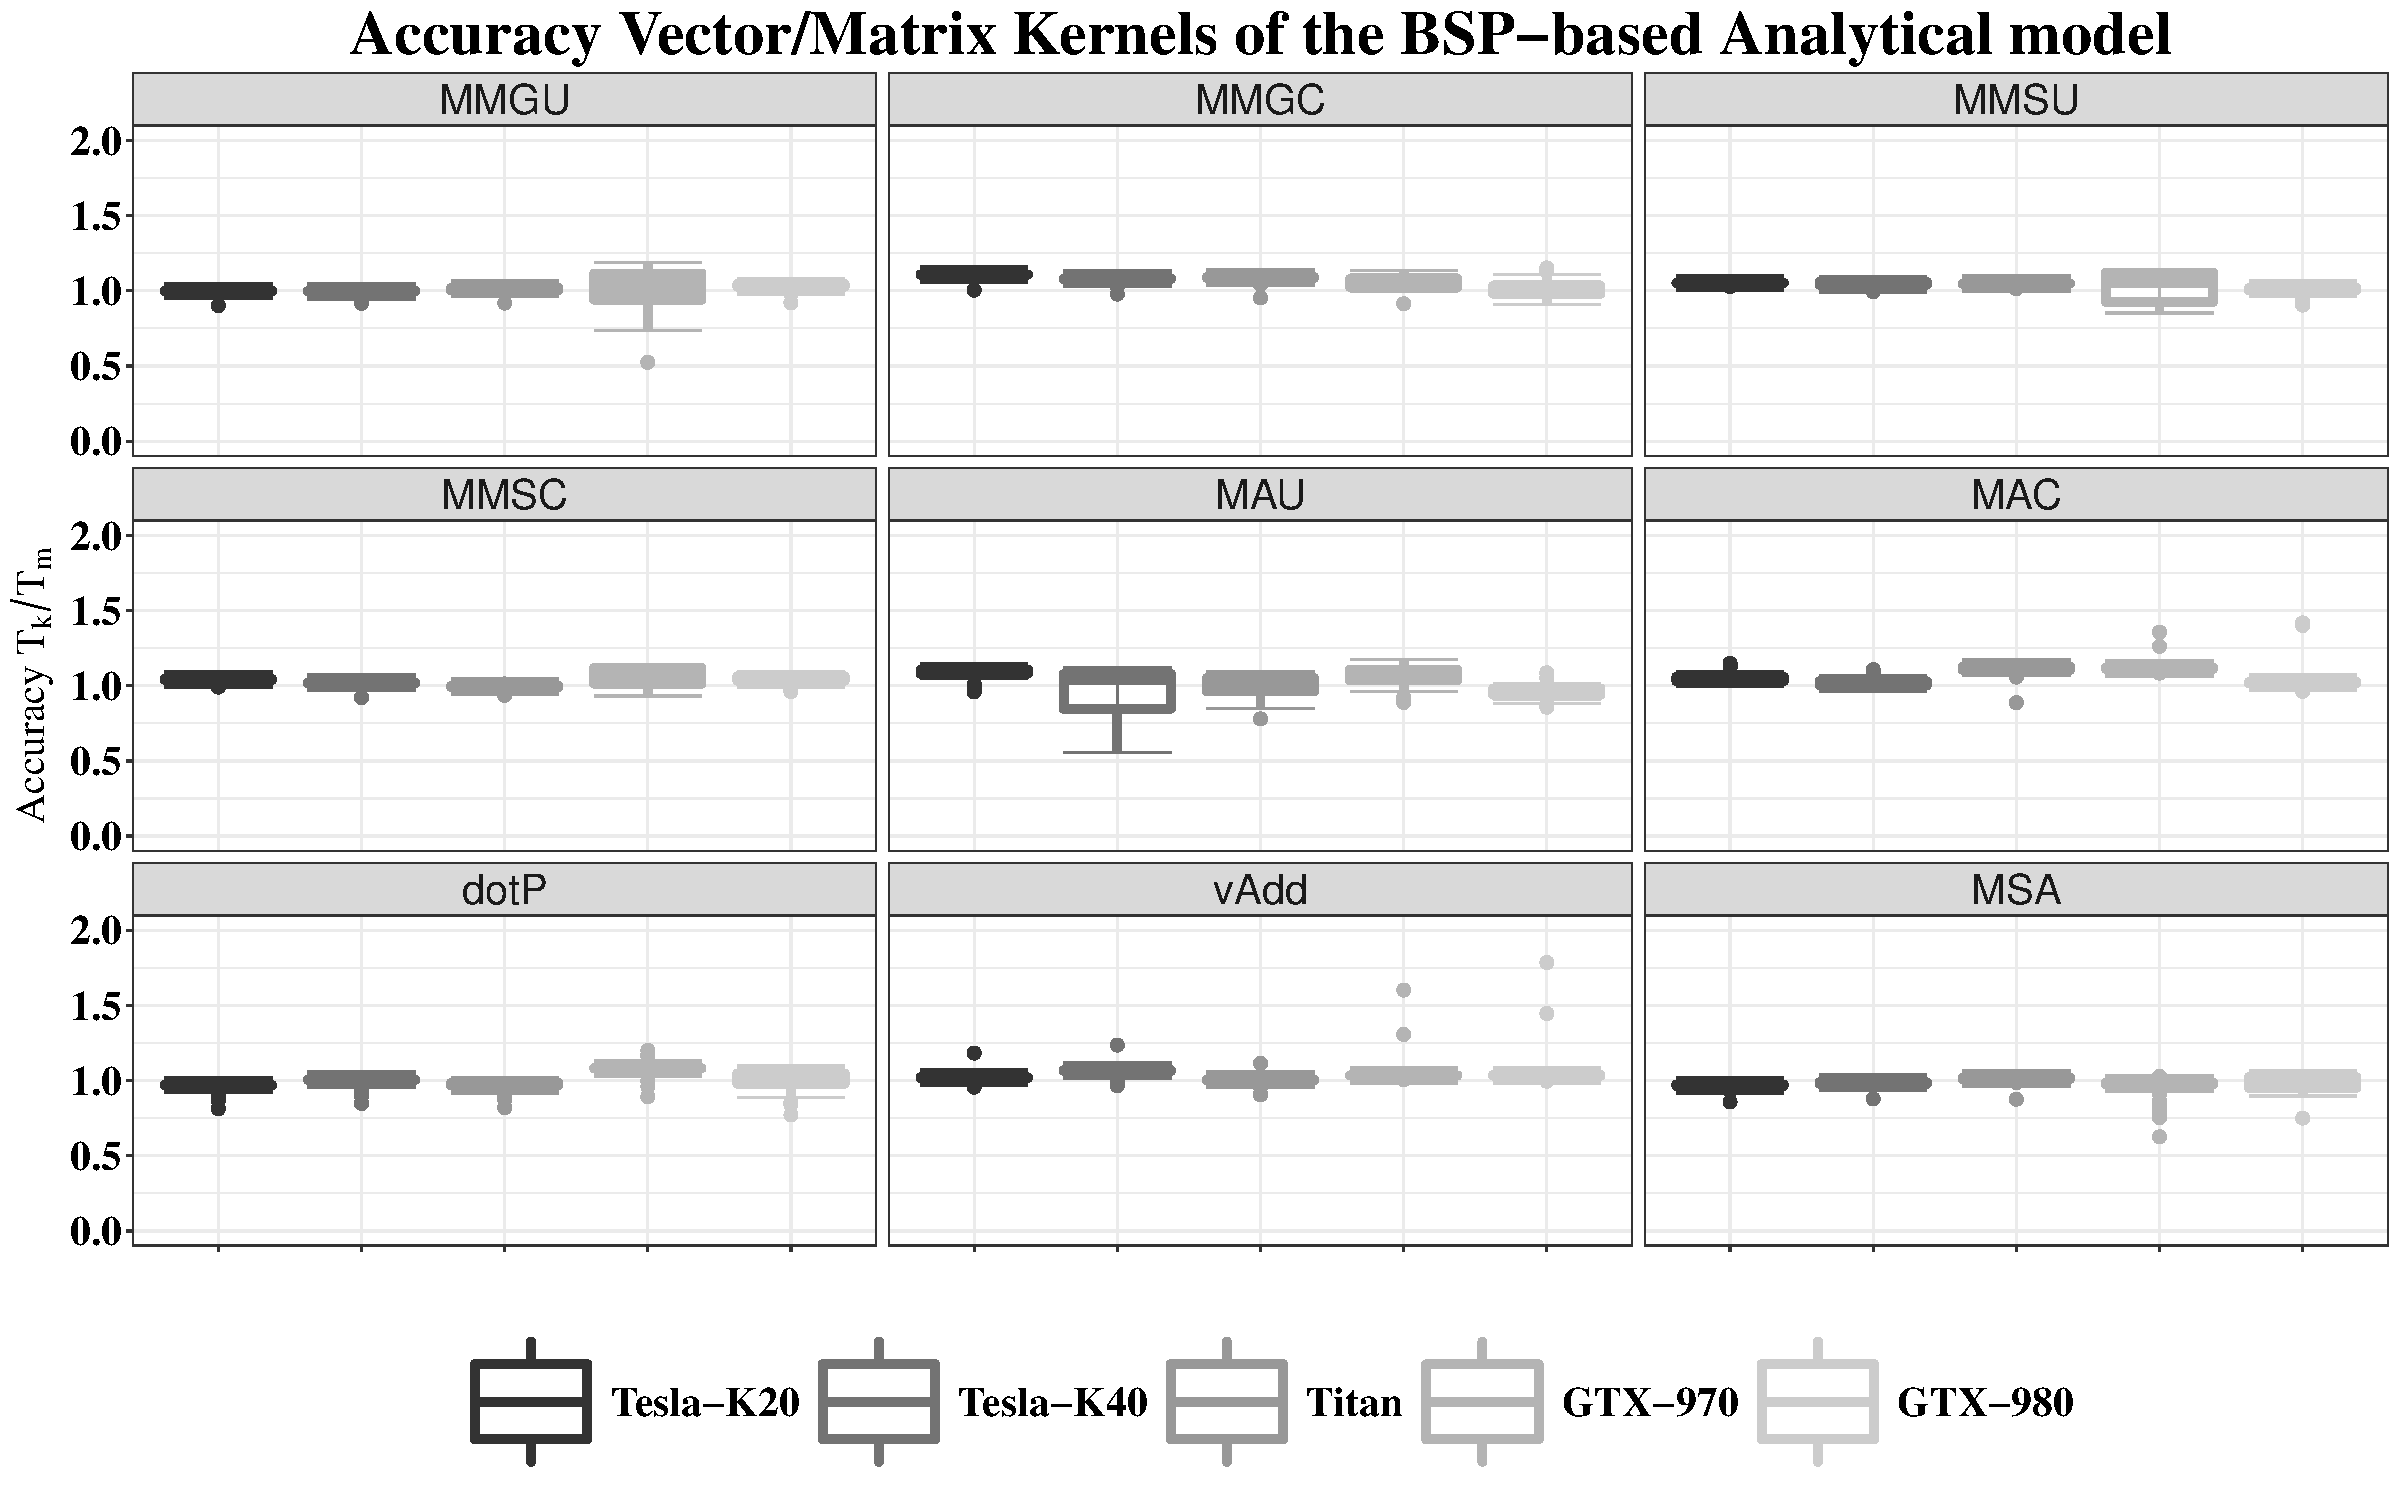
\includegraphics[scale=.4]{./images/ResutAnalyticalModel.pdf}
\caption{$T_k/T_m$  of vector and matrix algorithms with different values of $\lambda$, see table~\ref{tab:Lambda-NCA}}
\label{fig:resultsVMApp}
\end{figure}


Figure~\ref{fig:ResultsRodinia} shows the rate between the predicted and measured times of each one of the selected Rodinia CUDa kernels for the all the GPUs. This figure shows that predictions of the kernels BCK-1, BCK-2, HTW and HOT were between 0.9 and 1.1, showing a good prediction capability of the model. It was not possible to predict correctly the execution times of the kernels (GAU-1) and (GAU-2) because in both kernels the number of threads decrease in a loop during the execution of whole application. In both kernels execution around 10 threads are launched. GAU-K1 and GAU-K2 in each iteration of their execution decrease the number of threads and consequently the number of instructions. These instruction variations degraded the throughput significantly and the model required calibration of the parameter $\lambda$ or another adjustable parameter. These samples of GAU-K1 and GAU-K2 represented in big outliers and we have decided solve it in a future, adding parameters based on throughput. 

\begin{figure}[htpb]
\centering
 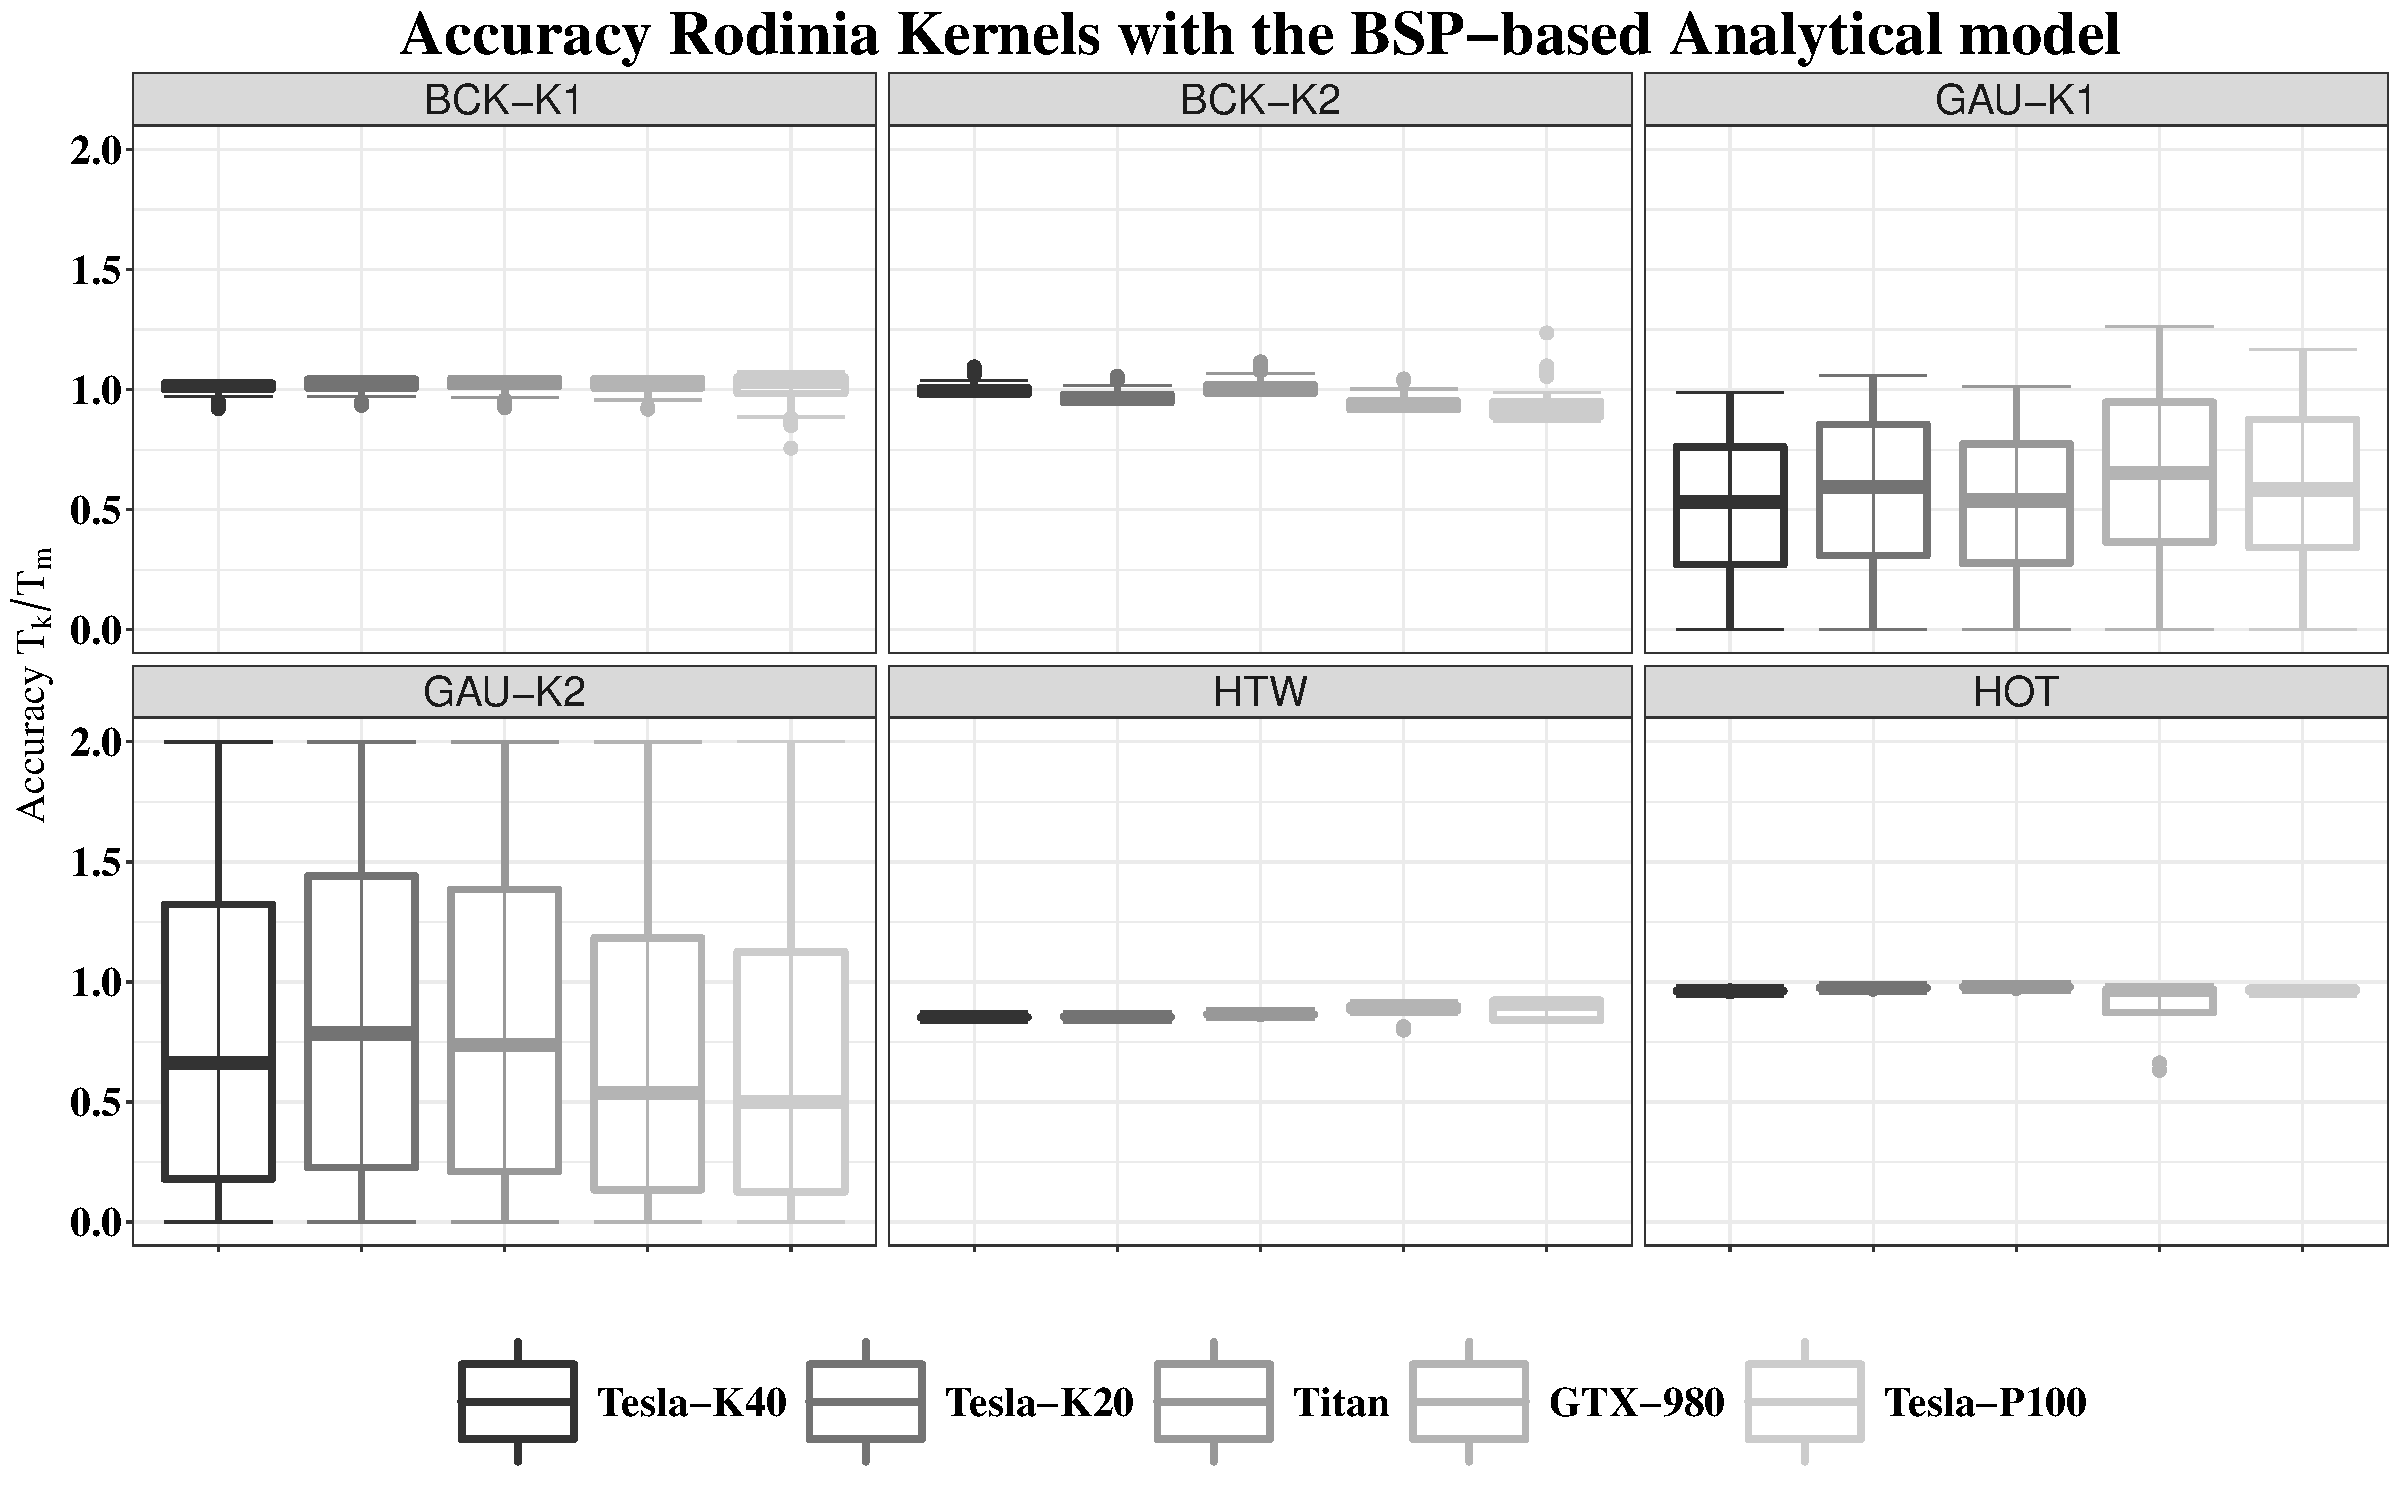
\includegraphics[scale=.4]{images/ResutAnalyticalModelRodinia.pdf}
\caption{$T_k/T_m$  of Rodinia CUDA kernels with different values of $\lambda$, see table~\ref{tab:lambdaRodinia}}
\label{fig:ResultsRodinia}
\end{figure}


These results show that we can use the model in the scenarios with different GPU types of the same architecture and with only one GPU type. In both cases the model can predict applications execution time from measurements on a single board with a single input size. With different GPU types, the prediction is less precise, since the optimal $\lambda$ value is different for each board. But it can still produce adequate predictions.

By considering two levels of memory, shared and global memories, we could accurately model the performance of these applications using several GPU models and problem sizes. The usage of two adaptable parameters $\lambda$ was sufficient to model the effect of data coalescing during read and write operations to the global memory. A similar set of parameters also model the effects of cache hits, computation and communication process of any GPU application. In the majority of the scenarios, the time measured were around $0.8$ to $1.2$ times the model predicted execution time. 

Next section will present some main related works using analytical model to predict GPU applications.
